\documentclass[conference]{IEEEtran}

\usepackage{graphicx}
\usepackage{amsmath}

\title{Membership Inference Resistance via Confidence-Aware Distillation}

\author{
\IEEEauthorblockN{Joseph D. Janicki}
\IEEEauthorblockA{
University of Mississippi \\
joseph.d.janicki@gmail.com
}
}

\begin{document}

\maketitle

\begin{abstract}
Membership inference attacks (MIA) pose a privacy risk in machine learning systems by enabling adversaries to determine whether a data sample was part of the original training dataset. While prior work has demonstrated strong attack performance under certain conditions, the effectiveness of these attacks depends on model behavior and dataset attributes. In this work, we study the conditions under which membership inference attacks succeed and propose a defense pipeline based on teacher-to-student distillation, combined with confidence-aware label processing and feature-level anonymization.

We begin by evaluating a range of attack strategies, from simple confidence-threshold methods to advanced shadow-model attacks. Our results show that naive attacks fail to detect meaningful leakage, while a carefully constructed Shokri-style shadow attack reveals measurable vulnerability in overfit models (ROC AUC $\approx$ 0.58 on the Adult dataset). In contrast, models trained with early stopping or regularization exhibit near-random attack performance (AUC $\approx$ 0.51), highlighting the role of training dynamics in privacy leakage.

Building on these findings, we introduce a defense framework that transforms the training signal rather than modifying model architecture. Across configurations, student models reduce membership inference risk to near-random levels while preserving strong predictive performance. Confidence clipping achieves the best utility--privacy tradeoff.

These results demonstrate that membership inference vulnerability can be mitigated through data-centric transformations, providing a practical alternative to more complex privacy-preserving training methods.
\end{abstract}

\section{Introduction}
Machine learning models and AI trained on sensitive data are vulnerable to privacy attacks that exploit unintended memorization (overconfidence). One such class of attacks, known as membership inference attacks, attempts to determine whether a specific data sample was included in a model’s training dataset. This poses a significant risk in domains where training data contain personally identifiable or sensitive information, as successful attacks can reveal participation in datasets even with only black-box access to the model.
Prior work has demonstrated that MIA attacks can achieve high success rates under certain conditions, particularly when models are overfit or trained on high-capacity architectures. However, the effectiveness of these attacks depends heavily on the underlying model behavior and the evaluation methodology used. In many cases, simple attack strategies fail to detect meaningful leakage, while more advanced approaches are required to uncover subtle membership signals. They also assume access to a similar dataset as the target model. This raises two key questions: when does membership inference leakage actually occur, and how can it be reliably mitigated without sacrificing model utility?
In this work, we address both of these questions through an empirical study. First, we evaluate the effectiveness of MIA attacks across multiple model regimes, including overfit, early stop, and realistically regularized models. We show that naive attack methods fail to capture meaningful leakage, while a carefully constructed shadow model attack reveals measurable vulnerability primarily in overfit models. These results show the importance of both attack strength and training dynamics in assessing privacy risk.
Building on these insights, we propose a training pipeline that reduces membership inference leakage through a combination of teacher to student distillation, confidence-aware label processing, and feature-level anonymization. While training dynamics such as early stopping and regularization are shown to influence leakage, our approach focuses on modifying the training signal used to produce downstream models rather than introducing specialized architectures or formal privacy mechanisms.
We construct a grid of student models using different combinations of label-processing and feature-level transformations, including temperature smoothing, confidence clipping, and input anonymization. Each configuration is evaluated in terms of both predictive performance and resistance to MIA attacks, allowing us to analyze the tradeoff between utility and privacy across a range of defense strategies.
Our results demonstrate that the proposed defense pipeline significantly reduces membership inference leakage, with attack performance approaching random guessing across most student models, while maintaining strong task utility. These findings suggest that privacy protection can be achieved through manipulation of training data representations, providing an alternative to existing defense strategies.
The contributions of this work are as follows:
(1) a systematic evaluation of membership inference attack effectiveness across different model tuning
(2) an analysis demonstrating that overfitting is a primary driver of membership leakage
(3) the development of a teacher-to-student defense pipeline incorporating confidence-aware and feature-level transformations
(4) a study showing that this approach reduces attack success to near-random levels while preserving model performance.


\section{Related Work}
(2016) (information leakage bounds)
A prominent piece of work focuses on formal privacy guarantees through techniques such as differential privacy, as described in Deep Learning with Differential Privacy (Abadi et al., 2016). These methods provide theoretical bounds on information leakage by introducing noise during training. Although they offer strong guarantees, they come at the cost of reduced model utility (accuracy) and require careful tuning of privacy budgets, making them less practical in some real-world scenarios.
(2017) (core attack)
Membership inference attacks were first formalized by Membership Inference Attacks Against Machine Learning Models (Shokri et al., 2017), who demonstrated that an adversary with black-box access to a model can determine whether a data sample was included in its training set. Their approach relies on training shadow models to mimic the target model’s behavior and then using the resulting outputs to train an attack classifier. This work established the foundation for subsequent membership inference research. However, their results are strongest in settings with high model capacity, overfitting, and multi-class datasets, which may not generalize to more constrained or well-regularized scenarios (Our research heavily abuses those weaknesses).
(2018) (yes its just a GAN)
Defensive strategies have also been widely studied. One common approach is adversarial regularization, as introduced in Membership Privacy through Adversarial Regularization (Nasr et al., 2018), where a model is trained jointly with an adversary that attempts to infer membership. The model is penalized when the adversary succeeds, encouraging it to suppress membership signals during training. While effective, this approach requires modifying the training process and introduces additional complexity, including balancing competing objectives between utility and privacy. (introducing a more pronounced utility tradeoff, whereas our approach sustains strong predictive performance while achieving near-random attack effectiveness.)
(2019)
Another perspective on the effectiveness of MIA attacks is provided in Systematic Evaluation of Privacy Risks of Machine Learning Models (Jayaraman and Evans, 2019), which evaluates attack performance across a range of datasets, model types, and defense strategies. Their results show that attack success is highly dependent on factors such as overfitting, model complexity, and data distribution, and that many proposed defenses introduce significant tradeoffs between utility and privacy. This work highlights that membership inference risk is not uniform across settings and must be evaluated empirically rather than assumed, motivating the need for systematic analysis of both attack effectiveness and defense mechanisms. (a trend also reflected in our results, where leakage varies with training dynamics; however, our findings further suggest that near-random attack performance can be achieved with only minimal utility degradation)
(2021)
Subsequent work has explored variations of MIA attacks with reduced assumptions. Label-only attacks, such as those proposed in Label-Only Membership Inference Attacks (Choquette-Choo et al., 2021), demonstrate that attackers can infer membership using only predicted labels rather than full probability vectors. While these methods are appealing in more restricted threat models, they rely heavily on differences in model decision boundaries and are less effective when models generalize well or exhibit minimal confidence separation between training and test data. (a trend present even in a shokri-style attack)
More recently, data-centric approaches have been explored to preserve privacy. For example, anonymization methods using generative models based on diffusion techniques try to preserve task-relevant information while removing sensitive attributes. These methods focus on transforming the data representation itself rather than modifying model architecture. However, they are designed for specific data modalities and require complex generative modeling pipelines.
In contrast to prior work, this study focuses on understanding the role of training dynamics in membership inference leakage and introduces a practical defense pipeline that transforms the training signal via teacher--student distillation and confidence-aware processing. Prior observations that MIA attacks often exploit model overconfidence and memorization motivate a data-driven approach that directly modifies the confidence structure of model outputs. By combining insights from attack design and data transformation, our approach aims to reduce leakage without requiring architectural changes or formal privacy constraints, instead targeting key signals associated with membership inference vulnerability.


\section{Methodology}

\subsection{Datasets}
We evaluate our approach on the Adult Income dataset from the UCI Machine Learning Repository, a widely used benchmark for tabular classification. The dataset contains a mix of numerical and categorical features describing demographic and employment attributes, with the prediction task being to determine whether an individual’s income exceeds a specified threshold. 
Tabular data is a good use case for two reasons. First, it allows for meaningful feature-level transformations, such as generalization and anonymization, which are more difficult to apply within high-dimensional image domains. Second, tabular datasets often contain quasi-identifiers, making them relevant for privacy-focused analysis.
In addition to the Adult dataset, we used the CIFAR-10 dataset to analyze behavior in an image setting. CIFAR-10 is commonly used in membership inference research due to its multi-class structure and the higher-capacity models it requires. 
Higher capacity models ussually memorize more, making MIA attacks generally more effective. Multi-class outputs bring more probability distributions that attack models can exploit. overfitting produces a stronger signal between member and non-members. Including CIFAR-10 allows us to evaluate the proposed defense pipeline against stronger attack signals.
Prior to training, the dataset is preprocessed using standard techniques, including normalization of numerical features, one-hot encoding of categorical variables, and handling of missing values. The dataset is then split into training, validation, and test sets for model development and evaluation.


\subsection{Teacher Models}
We construct three variants of a baseline neural network model, referred to as Model A (the teacher models). Each variant is trained under different conditions to isolate how overfitting and generalization affect attack vulnerability.
The first variant is an intentionally overfit model, trained for an extended number of epochs with minimal regularization. This model achieves high training accuracy but exhibits a significant gap between training and validation performance, indicating strong memorization of the training data. This setting is meant to amplify signals for membership inference.
The second variant is a realistically regularized model that incorporates dropout, batch normalization, weight decay, and early stopping. This model is designed to mimic realistic deployment conditions, maximizing generalization and minimizing the gap between training and validation performance. The idea is not just that it's realistic, but also that it has far weaker signals to attack, by reducing the validation gap.
The third variant is an early-stop model, which uses the same architecture as the overfit model but is trained for a limited number of epochs to maintain a minimal generalization gap. This configuration is intended to maintain constant capacity while reducing the validation gap. The model shows how much the architecture matters vs the validation gap and overfitting.
By comparing these three variants, we can analyze how training dynamics, rather than architecture, influence membership inference vulnerability. This controlled setup forms the foundation for both attack evaluation and defense development in subsequent sections.
In the figures below you can see model tuning and overfitting for comparison on their defense results.

\begin{figure}[htbp]
\centering
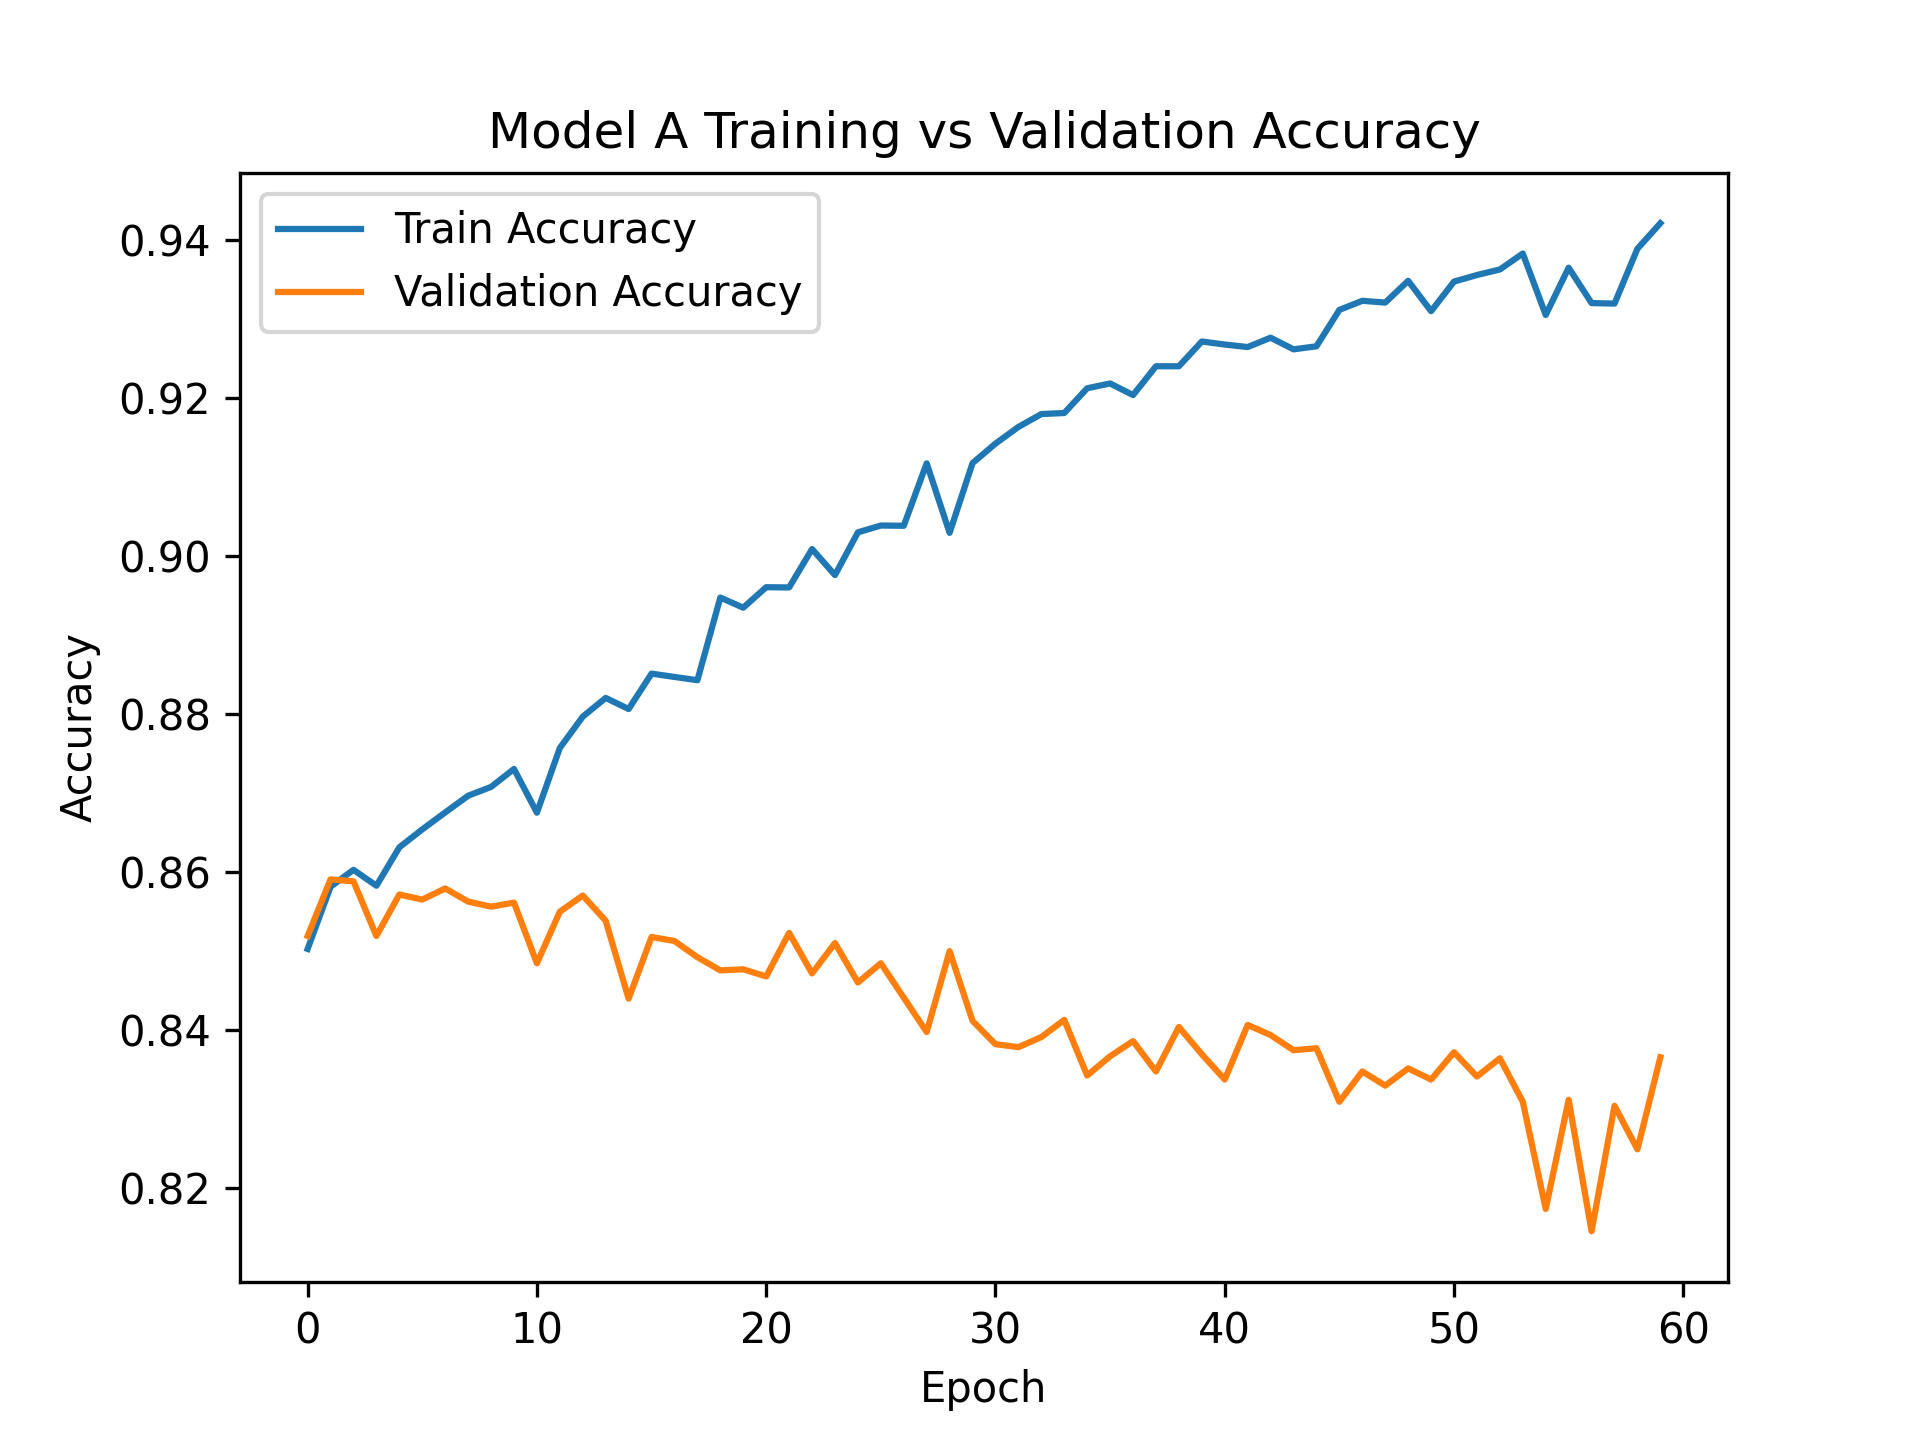
\includegraphics[width=0.45\textwidth]{modelAAccuracy.png}
\caption{Training vs validation accuracy for overfit adult model.}
\label{fig:modelA-overfit}
\end{figure}

\begin{figure}[htbp]
\centering
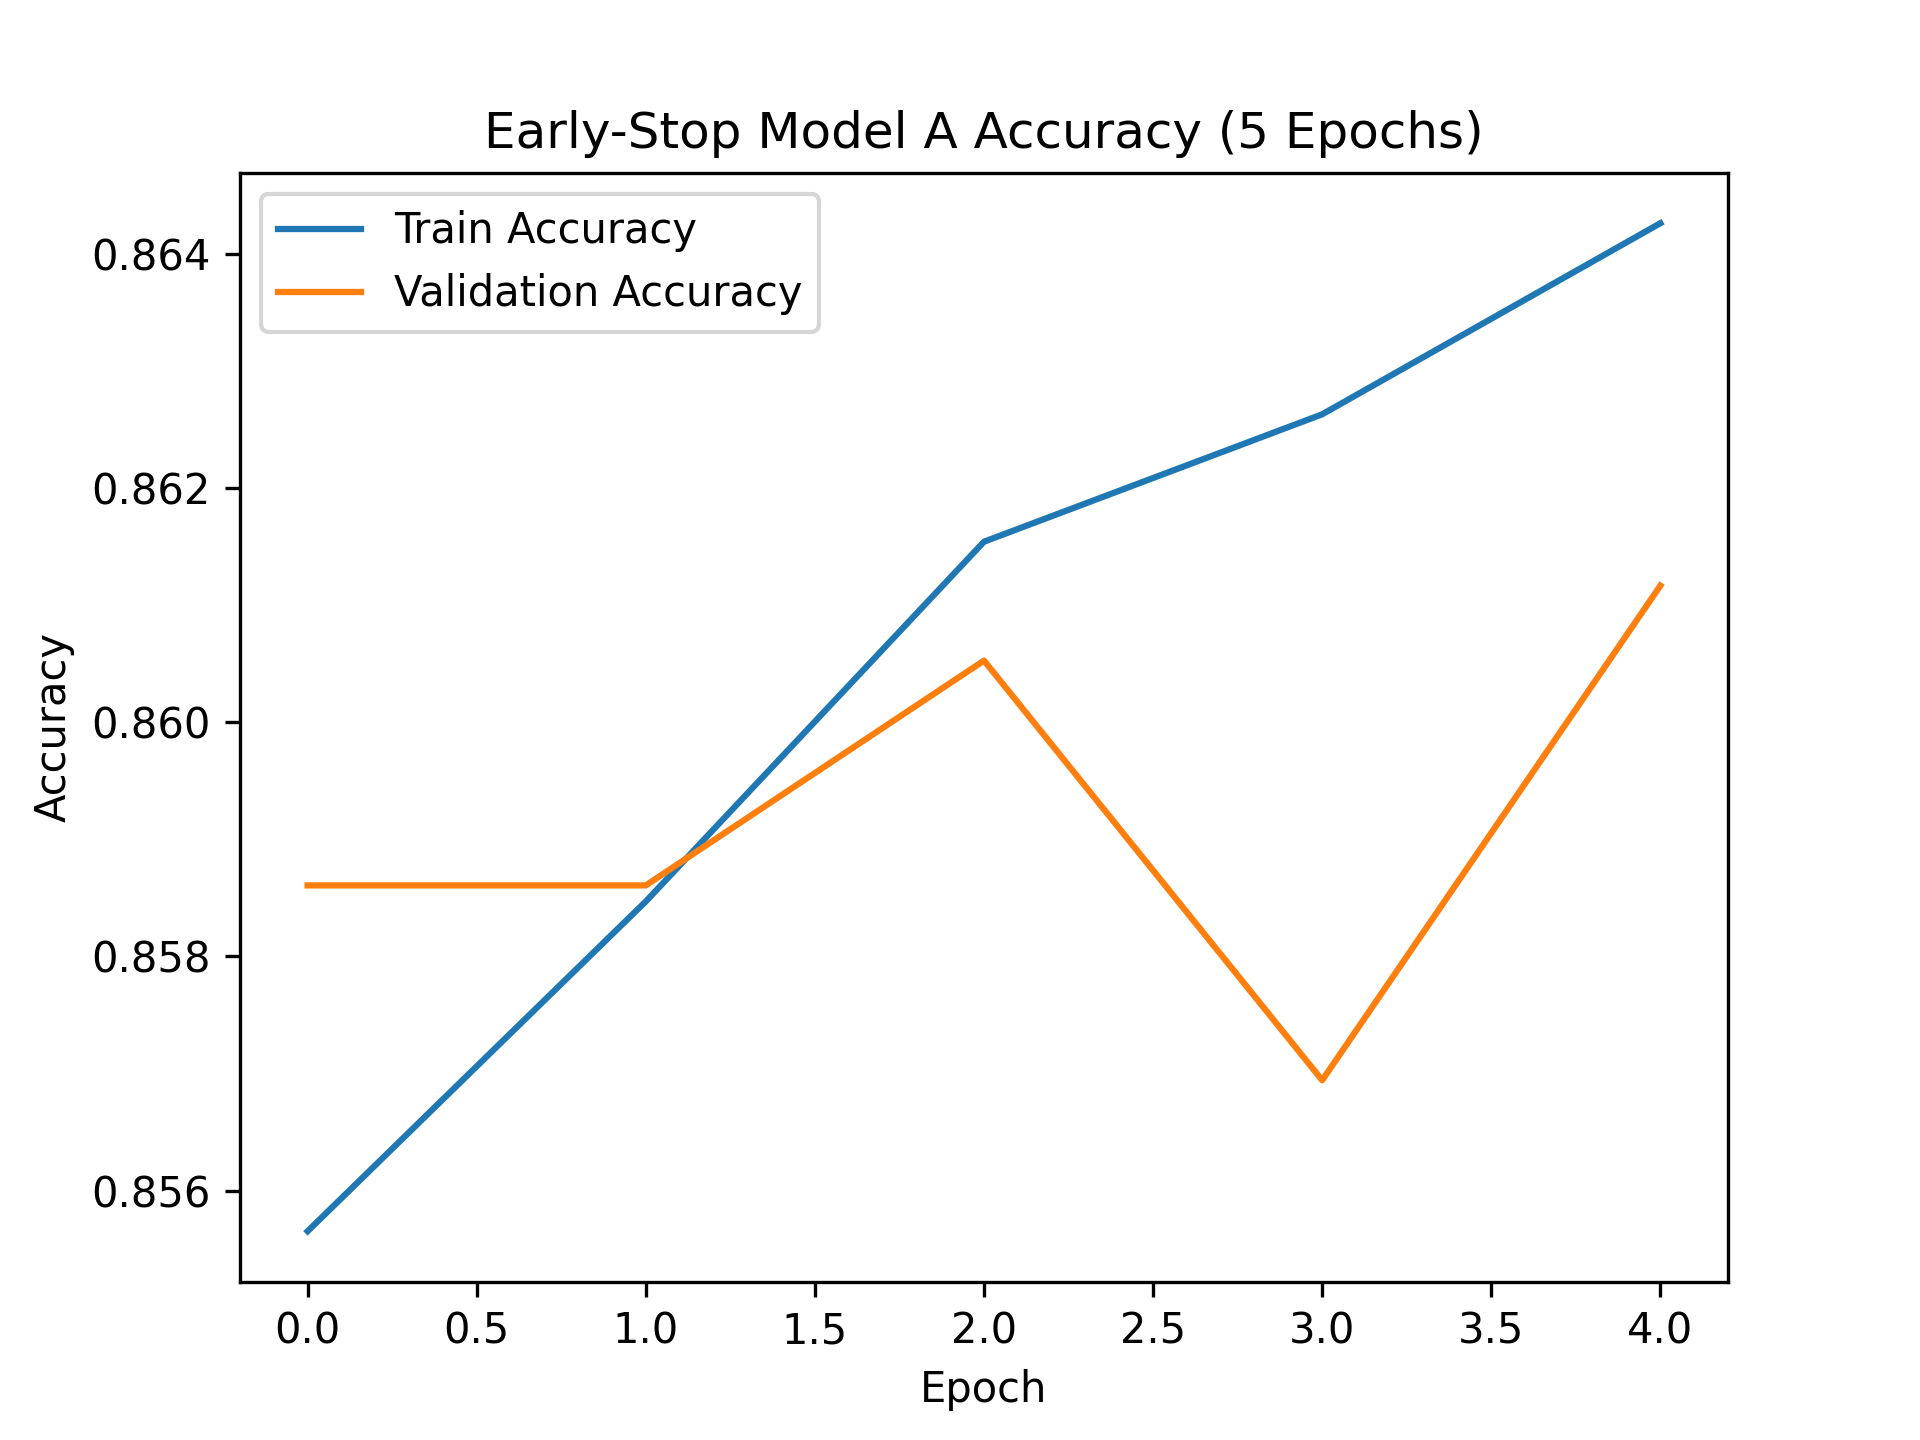
\includegraphics[width=0.45\textwidth]{modelaearlystopacc.png}
\caption{Training vs validation accuracy for overfit ault model stopped at 5 epochs.}
\label{fig:modelA-early-stop}
\end{figure}


\begin{figure}[htbp]
\centering
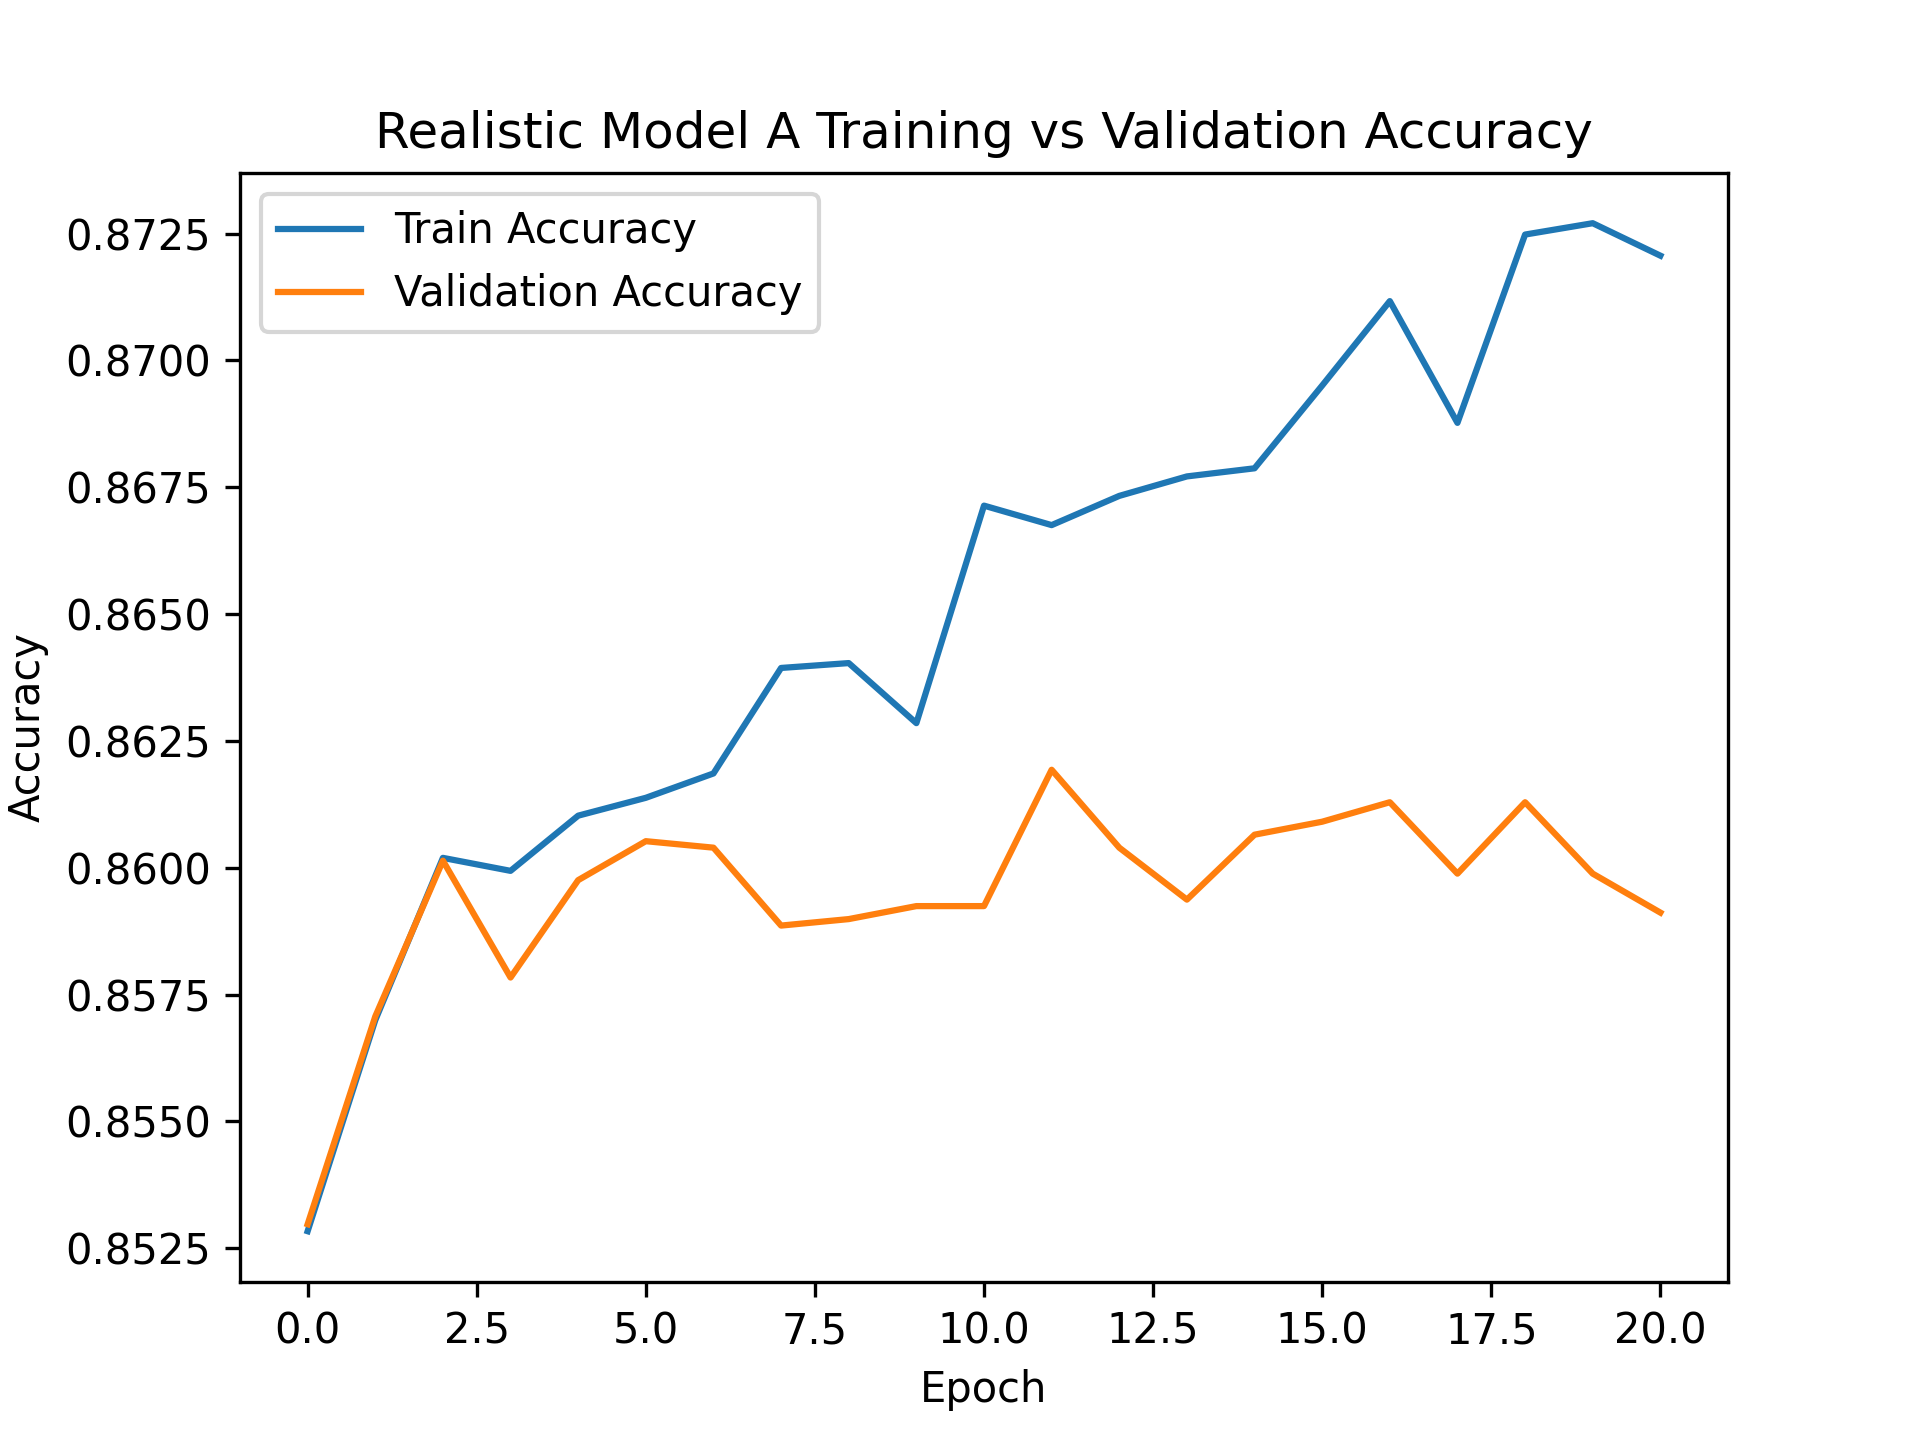
\includegraphics[width=0.45\textwidth]{modelarealisticacc.png}
\caption{Training vs validation accuracy for realistic adult model.}
\label{fig:modelA-realistic}
\end{figure}

\subsection{Membership Inference Attack Pipeline}
To evaluate leakage, we implement a series of MIA attacks of increasing complexity. This progression is designed to assess not only whether leakage exists, but also to incrementally attack the models.
We begin with a baseline confidence-threshold attack, classifying samples as members or non-members based on the model’s maximum prediction confidence (the hypothesis is that it wouldn't work). It proved ineffective in attacking the teacher models. Even after correcting for dataset imbalance, the attack achieves near-random performance (ROC AUC $\approx$ 0.50) across all model variants, indicating that confidence alone is not a reliable signal for membership inference in this context.
To capture more nuanced behavior, we took a step towards Shokri’s methods and implemented a shadow-model-based attack following the general framework introduced by Membership Inference Attacks Against Machine Learning Models (Shokri et al., 2017), a simpler version. In this approach, shadow models are trained to approximate the target model's behavior, and their outputs on member and non-member samples are used to train an attack classifier. An initial implementation using only raw class probabilities also fails to reveal meaningful leakage, suggesting that richer representations are required.
We extend the attack model and add additional behavioral features from model outputs. These include prediction entropy, confidence margin, loss with respect to the true label, and correctness indicators. This feature-aware attack improves performance on the overfit model (AUC $\approx$ 0.57 on the adult dataset) while remaining near-random for early-stop and realistic models. This result indicates that leakage is present, but that less vulnerable models require more expressive features.
Finally, we implement a Shokri-style attack with regime-matched shadow models and class-specific attack classifiers. This configuration aligns the training conditions of shadow models with those of the target model and accounts for class-dependent leakage patterns. This version achieves the strongest results, with the overfit model reaching AUC $\approx$ 0.58 (on the adult dataset), while other models remain near random ($\approx$ 0.51). Additional extensions, including expanded feature sets and alternative classifiers such as Random Forests, yield diminishing returns and sometimes worse attacks, suggesting that the primary leakage signal is already captured.
Building this attack leads to two key findings. First, weak attacks fail to detect membership inference leakage even when it exists. Second, leakage is strongly influenced by training dynamics, with overfitting producing measurable signals while well-generalized models resist even realistic threat models.

\subsection{Student Defense Pipeline}
To mitigate inference leakage, we propose a defense pipeline that trains student models (Model B) using transformed synthetic data generated by the teacher model (Model A). Rather than modifying the model architecture or training objective, this approach directly acts on the training signal to suppress features with overconfident and memorized signals.
The pipeline begins with the teacher generating synthetic training labels. sigmoid + BCE-style output was used with the teacher to produce a probability distribution over classes. From there, a set of label-processing strategies is used to modify the generated samples. These include raw soft labels, temperature-scaled soft labels, confidence-clipped probabilities, and hard labels derived from the maximum-probability class (think arg max). Each transformation adjusts the confidence structure of the training signal to reduce overconfident predictions.
After label processing, we apply further transformations to the input data, including anonymization via feature generalization and filtering of high-confidence samples. In the adult dataset, a threshold is used; in CIFAR-10, because the overfit model is too confident, a percentage of the highest confidence scores is discarded. Feature generalization reduces the specificity of input attributes, limiting the model’s ability to memorize unique patterns, while confidence-based filtering removes samples that are most likely to carry strong membership signals.
By combining these strategies, we construct a grid of label-processing and feature-level defense combinations to train the students on. For the Adult dataset, this yields 12 distinct configurations across four label modes and three feature modes. Each configuration is used to train a separate student model with the same base architecture, allowing for controlled comparison across defense strategies.
All student models are evaluated against the original ground-truth labels to measure task utility, rather than against the teacher-generated labels used during training, ensuring true predictive capability rather than mere mimicry of the teacher model. MIA attacks are then applied to each student model using the validated third variation attack.
This design allows us to analyze the tradeoff between utility and privacy, and to identify defense strategies that effectively reduce leakage while preserving model performance.

\section{Evaluation}

\subsection{Metrics}
Model accuracy is measured using classification accuracy and F1 score against the original ground-truth labels. This ensures that performance reflects true predictive capability rather than agreement with teacher-generated labels.
Privacy risk is evaluated using MIA attacks, with performance measured using the Area Under the Receiver Operating Characteristic Curve (ROC AUC). Unlike accuracy, which depends on a specific decision threshold, AUC measures the attack model’s ability to distinguish between member and non-member samples across all thresholds.
Accuracy alone can be misleading in this setting, particularly when the attack dataset is imbalanced. For example, an attack model that predicts all samples as members may achieve high accuracy while failing to learn a meaningful distinction. AUC provides a more reliable measure of attack effectiveness by capturing the separability of the underlying score distributions.
Throughout this work, an AUC near 0.5 is interpreted as random guessing, indicating minimal membership inference leakage, whereas higher values indicate greater vulnerability. Values below 0.5 indicate attack instability. Theoretically (this isn’t yet tested), one might be able to flip the classes and turn that instability into a sort of reverse signal to infer members of the original data.

\subsection{Teacher Model Results}
We first evaluate MIA attacks on the Model A variants on to establish a leakage baseline. Using the strongest attack configuration, we observe a clear distinction between overfit and well-generalized models.
The overfit model exhibits the greatest leakage, achieving an attack AUC of approximately 0.58 on the adult dataset; on CIFAR-10, it is 0.68. In contrast, both the early-stop and realistically regularized models produce near-random attack performance, with AUC values close to 0.51. The CIFAR-10 set still has meaningful leakage when well-tuned, but it is massively reduced. These results indicate that overfitting is a primary driver of membership inference vulnerability, while models with small generalization gaps are significantly more resistant.
These findings also highlight the importance of attack strength. Simpler attacks fail to detect leakage even in the overfit model, while the Shokri-style attack reveals measurable signals. The absence of attack success under weak methods does not necessarily imply the absence of leakage.

\subsection{Student Model Results (Adult)}
We evaluate the predictive performance of all student models trained under the defense pipeline. Results are summarized in the arrow plot below
NOTE: Here, ‘original’ refers to the baseline preprocessed feature representation (e.g., normalized and encoded inputs), not the raw dataset.

Models trained on original feature representations consistently achieve the highest performance, with leakage closer to random guessing (Adult dataset, overfit teacher). The best-performing configuration, student\_clip\_soft\_original, achieves approximately 0.858 accuracy and 0.667 F1 score. Other original-feature variants, including student\_hard\_original and student\_temp\_soft\_original, perform similarly, with accuracies in the range of approximately 0.853--0.856.
Feature anonymization introduces a small performance reduction, with accuracy decreasing by approximately 1--2\% across configurations (Adult dataset). For example, student\_clip\_soft\_anon achieves approximately 0.846 accuracy. In contrast, filtering high-confidence samples results in a more substantial degradation, with accuracies dropping to approximately 0.816--0.829 due to the reduced number of training samples.
Across label-processing strategies, confidence clipping provides the most favorable balance, consistently achieving the highest or near-highest accuracy across feature modes. These results indicate that confidence-aware label transformations can preserve strong predictive performance while modifying the training signal.
All student configurations substantially reduce membership inference leakage compared to the overfit teacher model (Adult dataset, overfit Model A baseline AUC $\approx$ 0.58). Most student models achieve attack AUC values in a narrow range between approximately 0.50 and 0.53, indicating near-random attack performance. For example, student\_clip\_soft\_original achieves an AUC of approximately 0.518, while student\_temp\_soft\_original reaches approximately 0.527.
Feature anonymization provides a small but consistent reduction in attack performance, with AUC values typically around 0.513--0.515. In contrast, filtered variants produce unstable or below-random AUC values (Adult dataset), such as 0.4017 and 0.3508, which indicate unreliable or inverted attack signals rather than meaningful improvements in privacy.
The best overall tradeoff is achieved by student\_clip\_soft\_original, which maintains high predictive performance ($\approx$0.858 accuracy) while reducing attack AUC to approximately 0.518 (Adult dataset, overfit teacher). Notably, all non-filtered student configurations reduce leakage to near-random levels while preserving strong utility, demonstrating the effectiveness of the proposed training-signal transformation approach.

\subsection{Student Model Results (CIFAR-10)}
We evaluate the predictive performance of all student models trained under the defense pipeline. Results are summarized in the arrow plot below
NOTE: Here, ‘original’ refers to the baseline preprocessed feature representation (e.g., normalized and encoded inputs), not the raw dataset.

Experiments on the CIFAR-10 dataset show that student models can maintain or even improve predictive performance while reducing membership leakage. In several configurations, student models trained on teacher-derived labels outperform their corresponding teacher models, particularly in the overfit setting, where student accuracy increases from 0.69 to the 0.75--0.77 range while AUC is reduced to near-random levels.
Both original and filtered feature variants often achieve comparable or improved performance relative to their teachers, while maintaining attack AUC values near 0.50. Notably, for the realistically trained CIFAR-10 teacher, the student\_hard\_filtered configuration achieves performance comparable to the teacher model while producing near-random AUC.
These results suggest that, when tuned, the proposed pipeline not only reduces leakage but can also improve generalization when the teacher model is overfit. Overall, the CIFAR-10 experiments demonstrate that the defense pipeline can achieve substantial privacy improvements with negligible performance impact, and in some cases, simultaneous gains in both utility and privacy.

\begin{figure}[htbp]
\centering
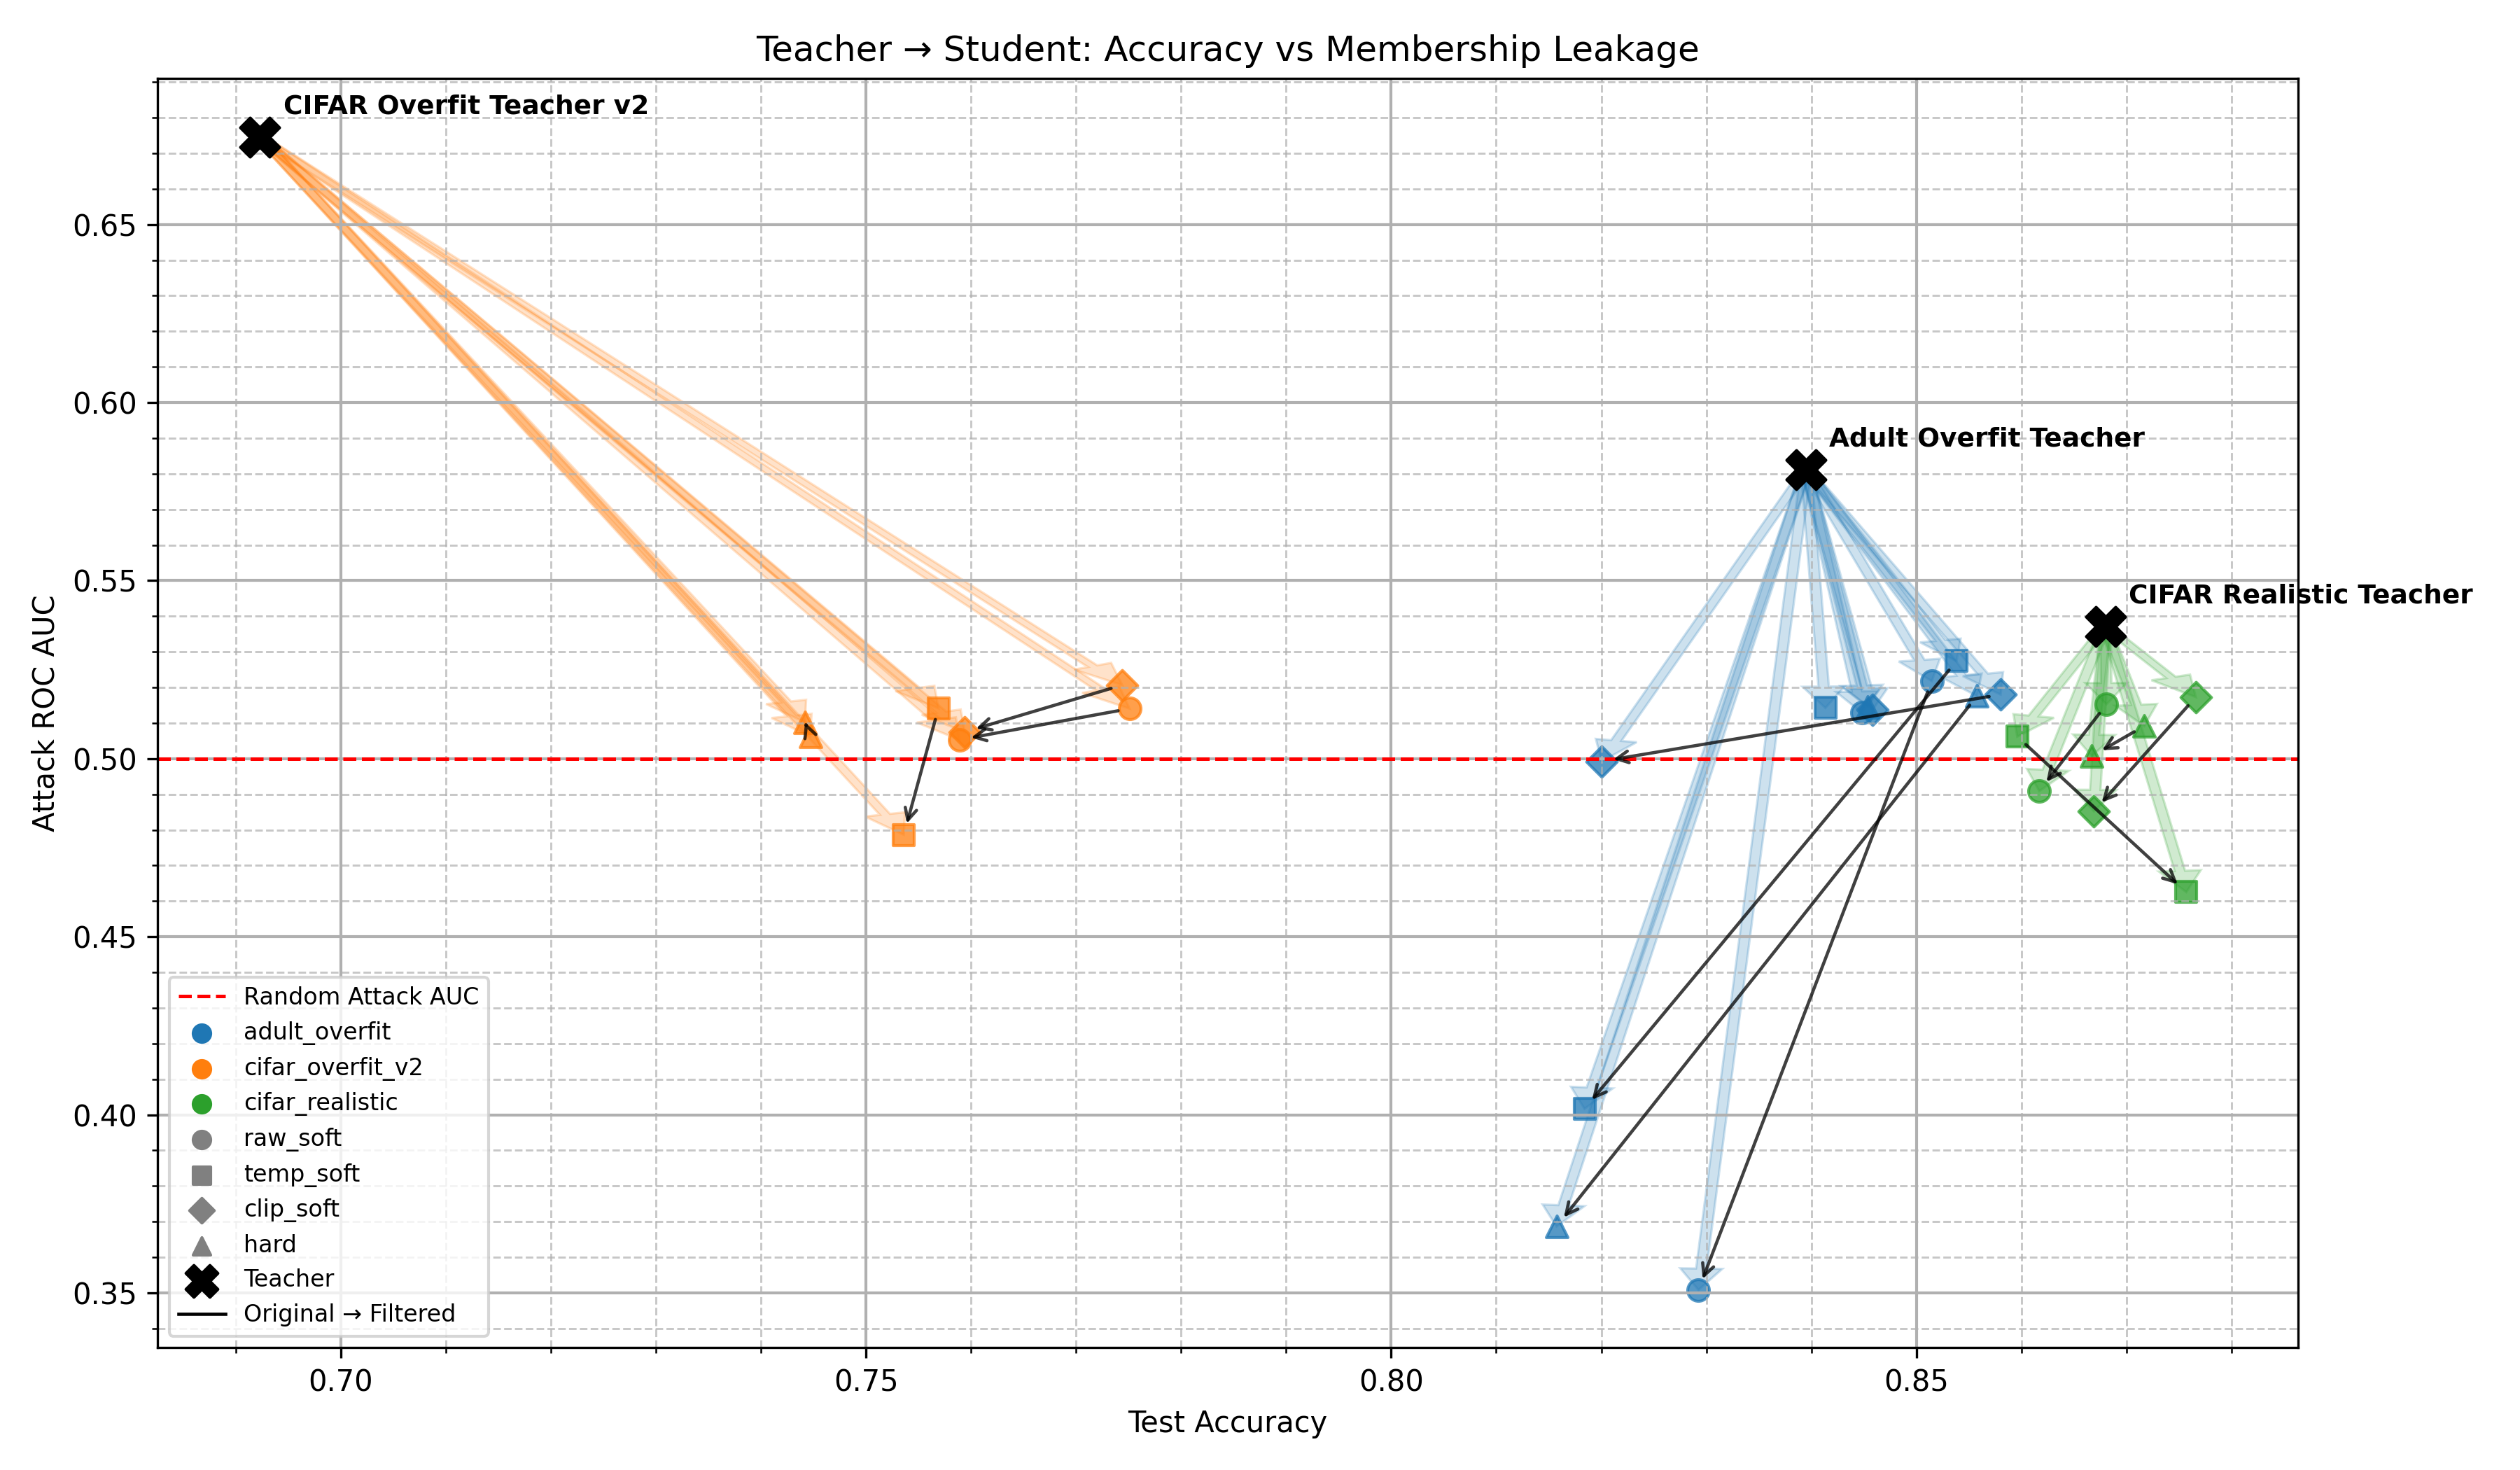
\includegraphics[width=0.45\textwidth]{arrowplot.png}
\caption{teacher to original student to filtered student}
\label{fig:arrowplot}
\end{figure}

\section{Conclusion and Future Work}
This work investigated the conditions under which membership inference attacks succeed and used that information to propose a practical defense pipeline that transforms the training signal with teacher--student distillation and confidence-aware processing. Through an evaluation of attack methods, we showed that weak attacks fail to detect leakage, while stronger shadow-model-based approaches reveal measurable vulnerability primarily in overfit models. These results confirm that membership inference risk is strongly influenced by confidence and training more so than model architecture.
Building on this, we introduced a defense framework that combines confidence-aware label transformations and feature-level processing to suppress membership signals. Across both tabular (Adult) and image (CIFAR-10) datasets, the proposed approach consistently reduced attack performance to near-random levels while maintaining strong predictive utility. On the Adult dataset, this was achieved with only a modest reduction in accuracy, while on CIFAR-10, student models were able to match or exceed teacher performance in several configurations while maintaining near-random attack effectiveness.
This demonstrates that effective mitigation of membership inference leakage can be achieved through data-centric transformations of the training signal, without requiring architectural changes or complex privacy-preserving training objectives. In particular, targeting overconfidence and training-specific memorization patterns provides a practical and scalable mechanism for reducing privacy risk.
Future work will focus on further refining the defense pipeline to achieve more consistent reductions in attack performance across all configurations while maintaining negligible impact on model utility. In particular, improving the stability of defense strategies, such as confidence filtering (tuning metrics like confidence thresholds and different percentage sample discarding) and better controlling the tradeoff between data reduction and performance, will be important directions. Additionally, scaling the approach to larger models and publicly deployed systems represents a key next step, as real-world applications often involve significantly higher-capacity architectures and more complex data distributions.
More broadly, extending this framework to modern large-scale models and evaluating its effectiveness in real-world deployment scenarios will help determine its practical viability as a general-purpose defense against membership inference attacks.


\section*{References}

\begin{thebibliography}{00}

\bibitem{shokri}
R. Shokri et al., ``Membership Inference Attacks Against Machine Learning Models,'' IEEE S\&P, 2017.

\bibitem{choquette}
C. Choquette-Choo et al., ``Label-Only Membership Inference Attacks,'' ICML, 2021.

\bibitem{nasr}
M. Nasr et al., ``Membership Privacy through Adversarial Regularization,'' CCS, 2018.

\bibitem{abadi}
M. Abadi et al., ``Deep Learning with Differential Privacy,'' CCS, 2016.

\bibitem{jayaraman}
B. Jayaraman and D. Evans, ``Evaluating Differentially Private Machine Learning in Practice,'' USENIX, 2019.

\bibitem{ho}
J. Ho et al., ``Denoising Diffusion Probabilistic Models,'' NeurIPS, 2020.

\end{thebibliography}

\end{document}
